\chapter{Quantenpunkte}

\noindent Diese Arbeit beschäftigt sich mit der mathematischen Modellierungen der Spindynamik eines negativ geladenen
Quantenpunktes, deshalb ist es sinnvoll vorab zu klären, was ein Quantenpunkt überhaupt ist. Damit einhergehend lassen sich die hier angenommenen Modelle begründen.\\
\begin{figure}[h!]
    \centering
    %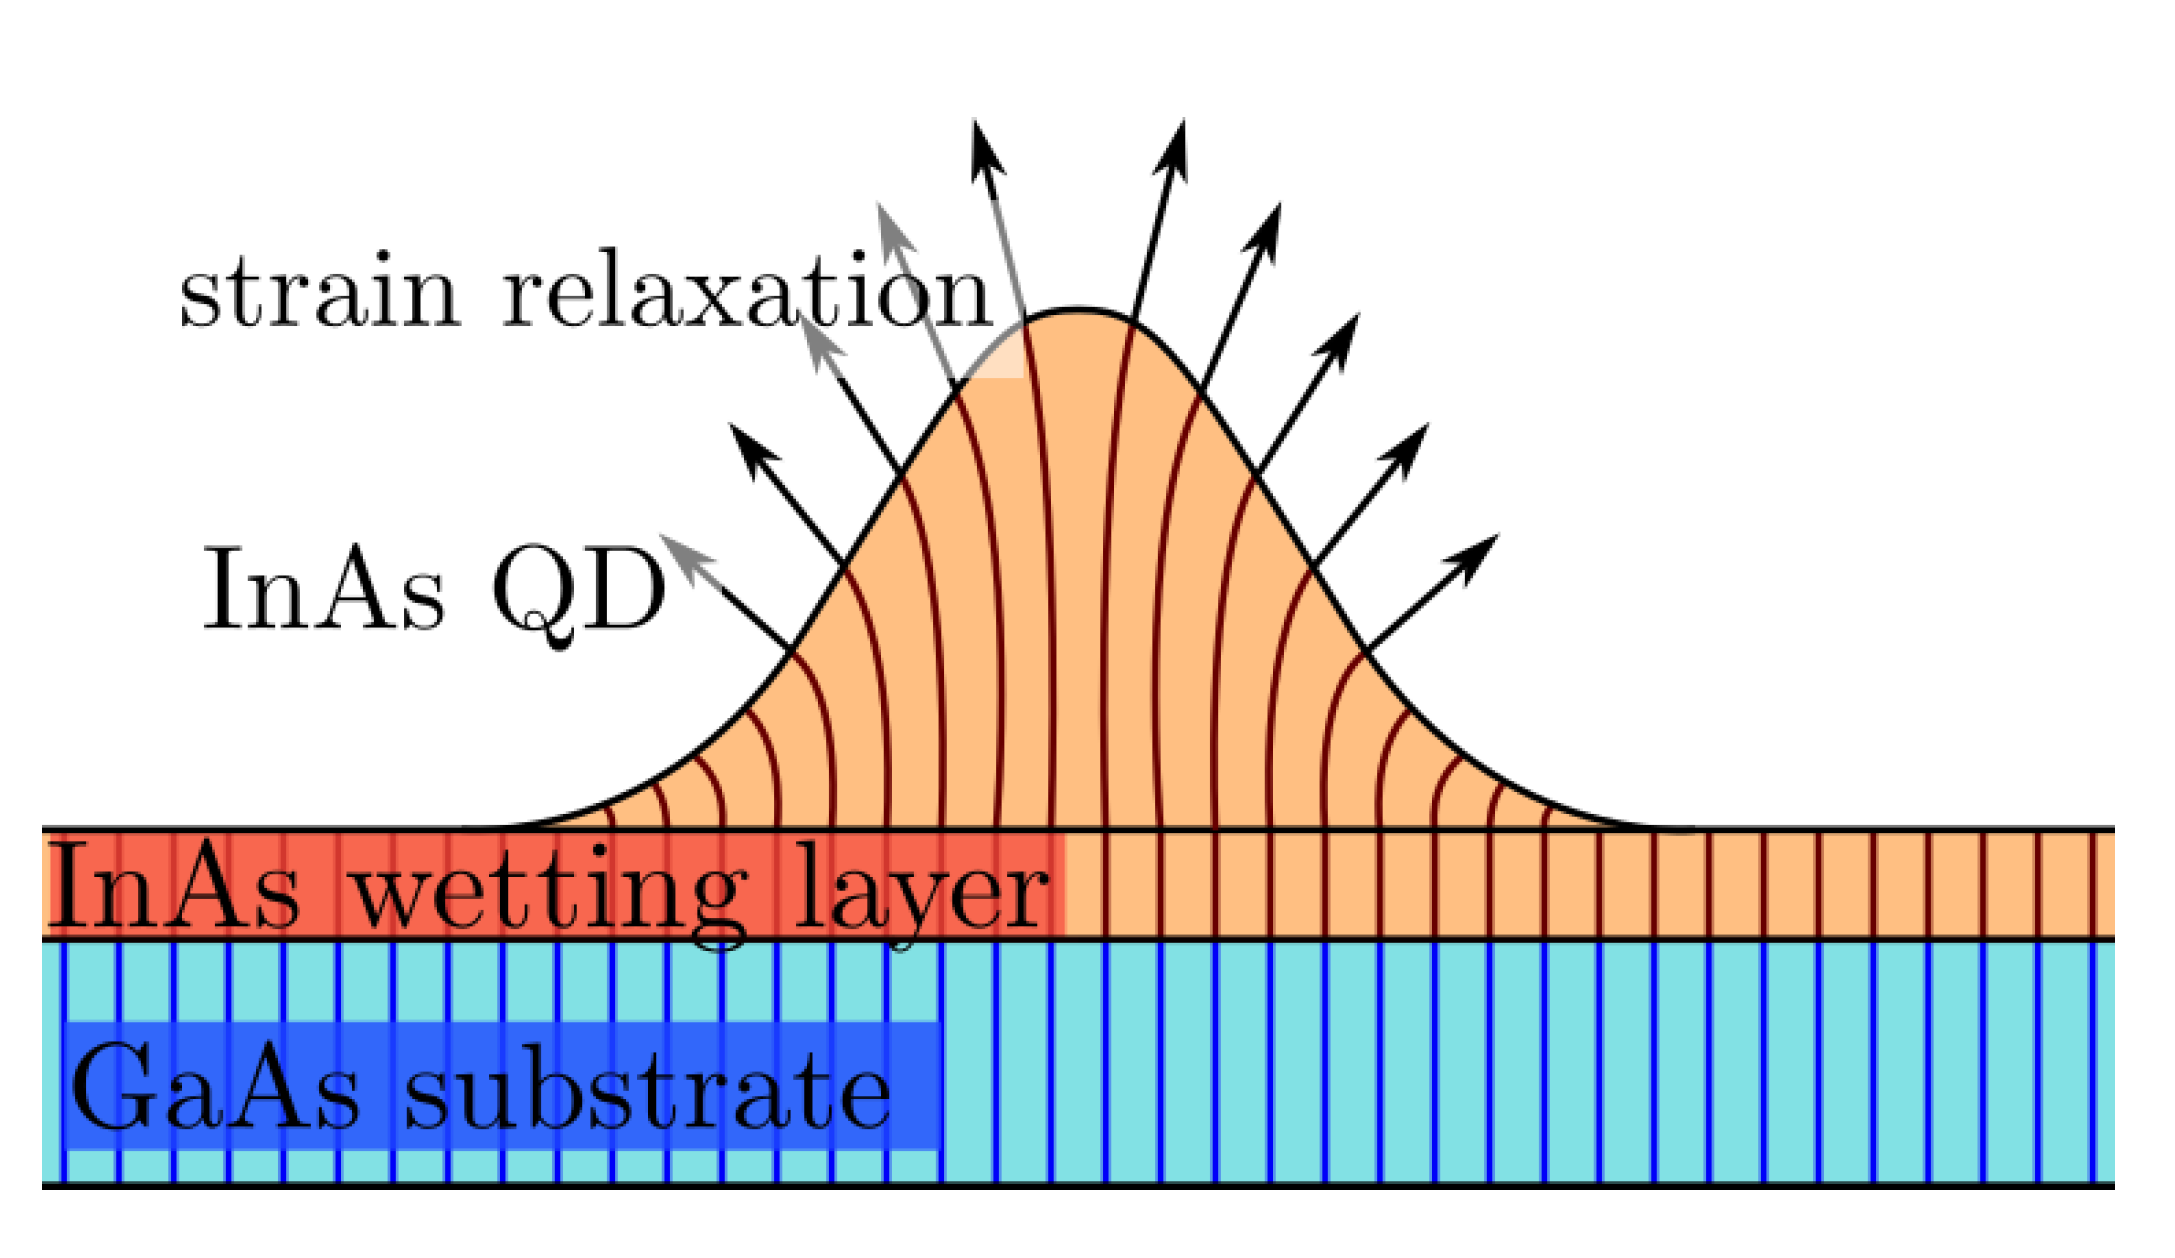
\includegraphics[width = 0.45\textwidth]{Abbildungen/QD_Schema.png}
    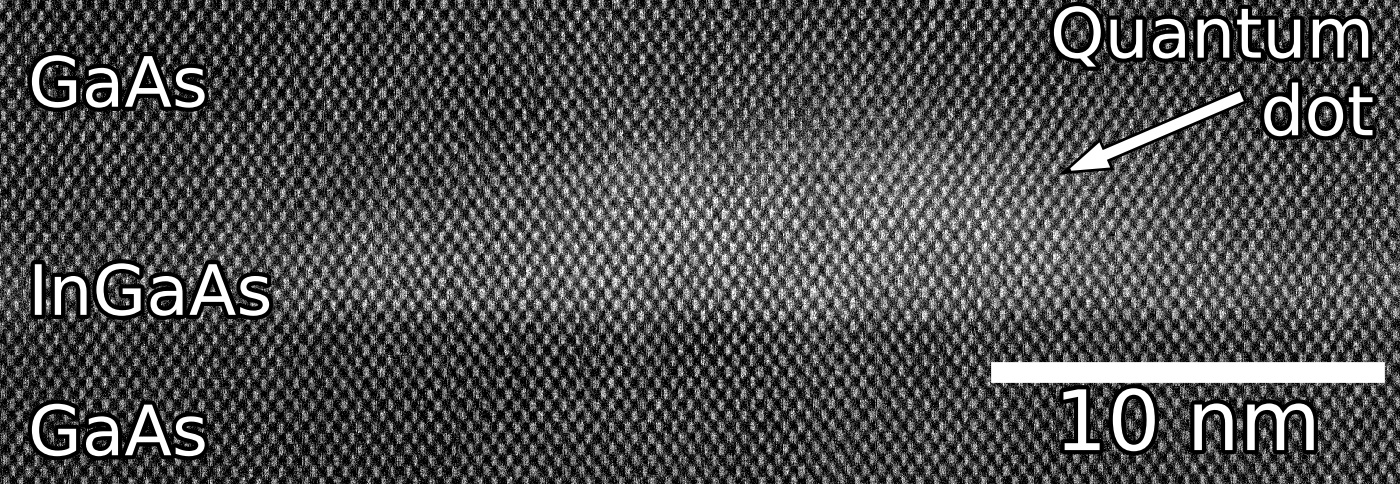
\includegraphics[width = 0.6\textwidth]{Abbildungen/Gaas_inas_quantum_dot_wikimedia.jpg}
    \caption{Ein atomar aufgelöstes Bild eines in Galliumarsenid (GaAs) eingebetteten Indium-Gallium-Arsenid (InGaAs)-Quantenpunkts. 
    Das Bild wurde mit der Rastertransmissionselektronenmikroskopie aufgenommen\cite{quantumdot_wikimedia}.}
    \label{fig:QD_Schema}
\end{figure}

\noindent Die hier betrachten Quantenpunkte sind nanoskopische Halbleiterstrukturen, die wie ein dreidimensionaler Potentialtopf fungieren
und einzelne Ladungsträger wie Elektronen oder Löcher einfangen können.\\
Die Stranski-Krastnov-Methode ist eine weitverbreitete Methode um Quantenpunkte zu erzeugen, dabei ist die Idee zwei Materialien mit 
unterschiedlicher Gitterkonstante mittels Molekularstrahlepitaxie aufeinander wachsen zu lassen. Der Kürze Halber lässt es sich 
beispielhaft an den beiden Materialien InAs und GaAs erklären, denn dabei wird eine InAs-Schicht auf ein GaAs-Substrat wachsen gelassen, 
wobei die Gitterkonstante des InAs etwa 7\% größer ist \cite{RevModPhys.85.79}, wodurch Spannung zwischen beiden Materialien entsteht. \\
\noindent Diese Spannung bewirkt eine Formationen von InAs-Inseln wie in \autoref{fig:QD_Schema} zu sehen, die nur wenige zehn 
Nanometer groß sind, und verändert selbst die elektronische Eigenschaften, hauptsächlich den elektrische Feldgradienten des 
Quantenpunktes. Nun wird GaAs auf das ganze Substrat gewachsen, so dass die InAs-Inseln vollständig von 
dem GaAs umschlossen sind. Diese umschlossenen InAs-Inseln bilden dann explizit den Quantenpunkt.\\
\begin{figure}
   \centering
    \includegraphics[width = 0.45\textwidth]{Abbildungen/QD_Energiebänder.png}
    \caption{Schematische räumliche Bandstruktur eines In(Ga)As/GaAs-Quantenpunktes mit den relevanten Bändern und einem 
    gefangenem Ladungsträger.}
    \label{fig:QD_Bandstruktur}
\end{figure}

\noindent Das GaAs, welches den In(Ga)As-Quantenpunkt umschließt, fungiert als Potentialtopf, denn die Energiebandlücke des InAs ist 
signifikant kleiner als die des GaAs. Nun kann ein einzelnes Elektron räumlich einfangen werden und durch die Lokalisierung 
die Wechselwirkung mit dem Substrat unterdrückt werden. Dadurch ist nur noch die Hyperfeinstruktur, also die Wechselwirkung mit den 
umliegenden Kernspins die dominante Wechselwirkung, wodurch die Dekohärenzzeit verlängert werden kann. Dies ist vorteilhaft, da 
eine kurze Dekohärenzzeit ein Hauptproblem bei der Realisierung des Quantencomputers ist.\\
In \autoref{fig:QD_Bandstruktur} ist zu erkennen, dass einzelne Elektronen (oder Löcher)
im InAs auf bestimmte Energieniveaus gefangen sind, ähnlich wie in einem Potentialtopf.\\
Quantenpunkte werden deshalb auch als \glqq künstliche Atome\grqq{} bezeichnet, da ganz in Analogie zu Atomen diskrete Enerigieniveaus 
von den eingefangen Elektronen besetzt werden können.
%B. Urbaszek, X. Marie, T. Amand, O. Krebs, P. Voisin, P. Maletinsky, A. Högele,
%and A. Imamoglu. Nuclear spin physics in quantum dots: An optical investigation.
%Rev. Mod. Phys., 85:79–133, 2013
%